\documentclass[11pt]{amsart}
\usepackage[margin=1in]{geometry}                % See geometry.pdf to learn the layout options. There are lots.
\geometry{letterpaper}                   % ... or a4paper or a5paper or ... 
%\geometry{landscape}                % Activate for for rotated page geometry
\usepackage[parfill]{parskip}    % Activate to begin paragraphs with an empty line rather than an indent
\usepackage{graphicx, enumerate}

\usepackage{amssymb}
\usepackage[normalem]{ulem}
\usepackage{epstopdf}
\DeclareGraphicsRule{.tif}{png}{.png}{`convert #1 `dirname #1`/`basename #1 .tif`.png}


\usepackage{tikz}
\usetikzlibrary{calc, through}
\usetikzlibrary{decorations.markings}
\usetikzlibrary{arrows}
\usetikzlibrary{positioning}

%\date{}                                           % Activate to display a given date or no date


\usepackage{hyperref}

%\newcommand{\deg}{\mathrm{deg}}

\newcommand{\bv}[1]{\ensuremath{\mathbf{#1}}}
\newcommand{\be}{\begin{enumerate}}
\newcommand{\ee}{\end{enumerate}}

\begin{document}
\begin{center}
\begin{Large} Math F307 \hfill Spring 2017

Homework Exercises 
\end{Large}
\end{center}
%\maketitle
%\section{}
%\subsection{}

\subsection*{Instructions for writing up homework}
\begin{itemize}
\item Although you are encouraged to work with your classmates on the homework assignments, you must write up the solutions individually.
\item Read the section!
 \item Use pen or non-smeary pencil. Do not have little scritchies on the side. 
 \item Staple your homework. 
 \item Write legibly, and leave lots of whitespace. Make sure your writing is dark enough to be readable. If this is problematic for you, consider typing your homework.
 \item Answer the question in complete sentences, where appropriate.
\item {\bf Write the \fbox{problem statements} as well as the answers. } This is not optional. \underline{Points will be deducted if you do not do this}.
\item Have headings indicating the section.
\item {\bf In the upper right hand corner of your top page,} write your name (first and last) on your assignment, along with the course number (Math 307) and which assignment it is.
\item {\bf You are expected to ask questions in class about the homework problems!}
\end{itemize}

\section*{Homework Set 8}

{\bf DUE Friday, March 24 \fbox{at the beginning of class}.}

You should {\bf read} each section!

\subsection*{Section 6.6}

To turn in: 10, 11, 13


\subsection*{Additional Problems}

Also turn in:
\be
\item Use Kruskal's Algorithm to find a minimal distance spanning tree for the graph shown in Figure \ref{Example1}. Draw in the edges of the spanning tree on a new copy of the  vertices. Break ties by choosing edges with a smaller-labelled endpoint.  Also provide a list of the edges in the order you added them.

\item  Use Prim's Algorithm to find a minimal distance spanning tree, {\bf starting at vertex 6} for the graph shown in Figure \ref{Example1}. Draw in the edges of the spanning tree on a new copy of the  vertices. Break ties by choosing edges with a smaller-labelled endpoint.  Also provide a list of the edges in the order you added them.

\item Use Dijkstra's Algorithm to find a minimal distance spanning tree for the graph shown in Figure \ref{Example1}, {\bf starting at vertex 0}. List all the vertices along with their distance from vertex 0. Also provide a list of edges in the order you added them.

\item Use Dijkstra's Algorithm to find a minimal distance directed spanning tree for the digraph shown in Figure \ref{Example1}, {\bf starting at vertex A}. List all the vertices along with their distance from vertex A. Are there any unreachable vertices (from A)? Which ones?

\item List the vertices of the tree shown in Figure \ref{tree} using the preorder traversal.

\item List the vertices of the tree shown in Figure \ref{tree} using breadth first search.

\item Label the vertices of the tree shown in Figure \ref{tree} using a topological ordering.

\item Find a topological ordering of the vertices of the digraph shown in Figure \ref{digraph}, or explain why no such topological sorting exists.

\item The ``while'' statement of the topological ordering digraph algorithm includes the statement that we can find a vertex $v$ with no incoming edges. Explain why, if every vertex of a digraph has at least one incoming edge, then the digraph must have a cycle.

\ee

%\subsection*{Tree Traversal Problems} 
%
%Think about, but do not turn in: 
%
%To turn in: 


%\subsubsetion{Dijkstra's Algorithm and Breadth First Search}

\begin{figure}[htbp]
\begin{center}
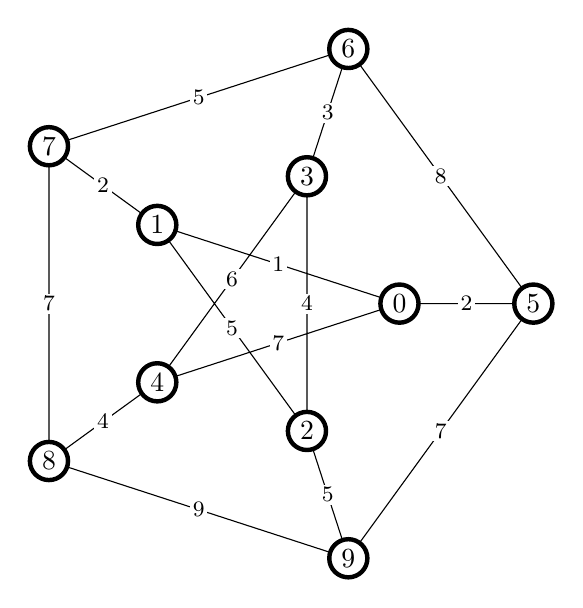
\begin{tikzpicture}[baseline=(current bounding box.center), scale=1.7]
\tikzstyle{graph}=[circle, draw, ultra thick, fill=black!0,
                        inner sep=2pt, minimum width=6pt]  ;
 \tikzstyle{la}=[midway, fill=black!0, font=\footnotesize, inner sep=1pt];
 %fontscale/.style = {font=\relsize{#1}]    ;
\foreach \i in {5,6,7,8,9}
{\coordinate (\i) at (\i*72:2);}
\foreach \j in {0, 1, 2,3, 4}
{\coordinate (\j) at (\j*72*2:1);}
\draw (1)-- (0) node[la] {1} -- (4) node[la] {7} -- (3)node[la]{6}  --(2) node[la] {4}  -- (1) node[la] {5} -- (0)  -- (5) node[la] {2} -- (6) node[la] {8} -- (7) node[la]{5} -- (8) node[la] {7} -- (9) node[la] {9} -- (5) node[la] {7} (6) -- (3) node[la]{3} (7) -- (1) node[la]{2} (8) -- (4) node[la]{4} (9) -- (2) node[la] {5};
\foreach \i in {0, 1, ..., 9}
{\draw (\i) node[graph] {$\i$};}
\end{tikzpicture}
\caption{Graph for Kruskal, Prim, and Dijkstra's Algorithm}
\label{Example1}
\end{center}
\end{figure}

\begin{figure}[htbp]
\begin{center}
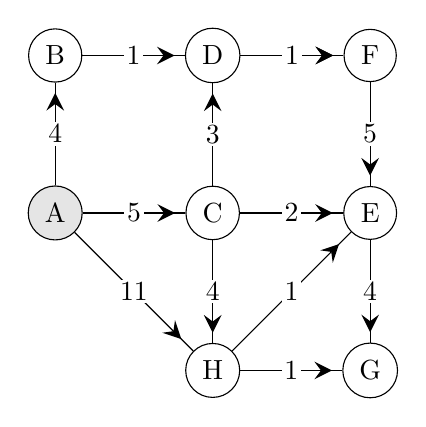
\begin{tikzpicture}[scale=2]
\tikzstyle{vtx}=[draw, circle, inner sep = 2 pt, node distance=4cm and 1.5 cm]
\tikzstyle{lbl}=[midway, inner sep = 1 pt, fill=white]
\tikzset{->-/.style={decoration={
  markings,
  mark=at position .9 with {\arrow[scale=2]{stealth}}},postaction={decorate}}}
\node[draw, circle, fill=gray!20] (A) at (1,0) {A} ;
\node[draw, circle] (B) at (1,1) {B} ;
\node[draw, circle] (C) at (2,0) {C} ;
\node[draw, circle] (D) at (2,1) {D} ;
\node[draw, circle] (E) at (3,0) {E} ;
\node[draw, circle] (F) at (3,1) {F} ;
\node[draw, circle] (H) at (2,-1) {H} ;
\node[draw, circle] (G) at (3,-1) {G} ;
%\draw (A) -- (B) node[midway, auto]{4} -- (D) node[midway, auto]{1}--(C) node[midway, auto]{3}--(E) node[midway, auto]{2}--(F)node[midway, auto]{5};
%\draw (A) -- (C) node[midway, auto] {5} -- (H) node[midway, auto] {4} -- (I) node[midway, auto] {1}-- (E) node[midway, auto] {4};
%\draw (D) -- (F) node[midway, auto]{1};\draw (H) -- (A)node[midway, auto]{11};
\foreach \i/\j/\k in {A/B/4, B/D/1, D/F/1, C/D/3, A/C/5, C/H/4, H/G/1, E/G/4, C/E/2, F/E/5, D/F/1, A/H/11, H/E/1}{
\draw[->-] (\i) --node[lbl]{\k} (\j);}
\end{tikzpicture}
\caption{A digraph}
\label{digraph}
\end{center}
\end{figure}


\begin{figure}[htbp]
\begin{center}
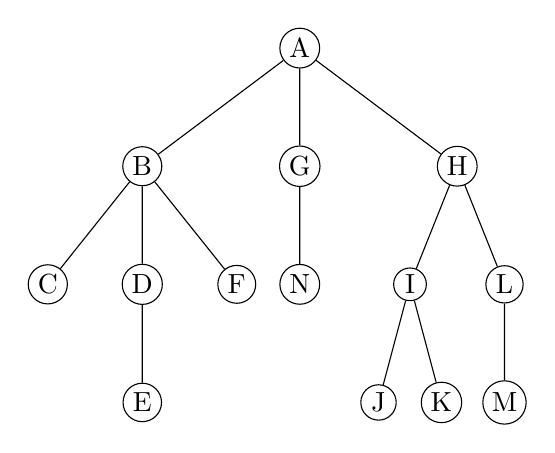
\begin{tikzpicture}[baseline=(current bounding box.center), scale=1, every node/.style={circle,draw},level 1/.style={sibling distance=20mm},level 2/.style={sibling distance=12mm}, level 3/.style={sibling distance=8mm}, inner sep =1.5pt
]
 \tikzstyle{la}=[midway, fill=black!0, font=\footnotesize, inner sep=1pt];
\node[] (A) {A}
 child[]{ node(B) {B}
 child{node (C){C}}
 child{node (D){D}
 child{node (E) {E}}
 }
 child{node (F) {F}}}
 child{node (G){G}
 child{node(N) {N}}}
 child{node (H) {H}
 child{node (I) {I}
 child{node (J){J}}
 child{node(K){K}}}
 child{node(L){L}
 child{node(M){M}}}};

\end{tikzpicture}
\caption{A tree}
\label{tree}
\end{center}
\end{figure}




\end{document}